% Graphic for TeX using PGF
% Title: /home/isobel/Documents/McMaster/PythonCodes/DataAnalysis/Doc/Design/MG/UseHierarchy_DataProcessing.dia
% Creator: Dia v0.97.2
% CreationDate: Mon Nov  6 23:35:15 2017
% For: isobel
% \usepackage{tikz}
% The following commands are not supported in PSTricks at present
% We define them conditionally, so when they are implemented,
% this pgf file will use them.
\ifx\du\undefined
  \newlength{\du}
\fi
\setlength{\du}{15\unitlength}
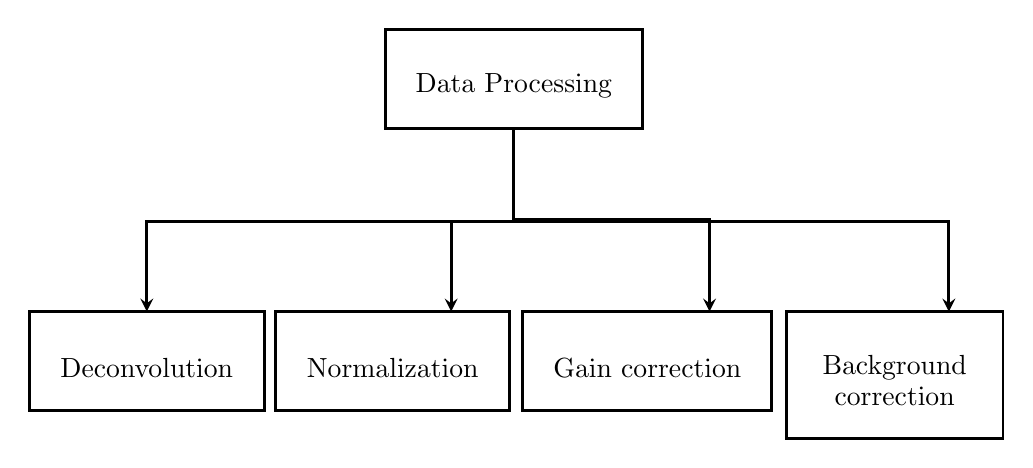
\begin{tikzpicture}
\pgftransformxscale{1.600000}
\pgftransformyscale{-1.600000}
\definecolor{dialinecolor}{rgb}{0.000000, 0.000000, 0.000000}
\pgfsetstrokecolor{dialinecolor}
\definecolor{dialinecolor}{rgb}{1.000000, 1.000000, 1.000000}
\pgfsetfillcolor{dialinecolor}
\definecolor{dialinecolor}{rgb}{1.000000, 1.000000, 1.000000}
\pgfsetfillcolor{dialinecolor}
\fill (22.901007\du,0.879365\du)--(22.901007\du,2.372698\du)--(26.768507\du,2.372698\du)--(26.768507\du,0.879365\du)--cycle;
\pgfsetlinewidth{0.070000\du}
\pgfsetdash{}{0pt}
\pgfsetdash{}{0pt}
\pgfsetmiterjoin
\definecolor{dialinecolor}{rgb}{0.000000, 0.000000, 0.000000}
\pgfsetstrokecolor{dialinecolor}
\draw (22.901007\du,0.879365\du)--(22.901007\du,2.372698\du)--(26.768507\du,2.372698\du)--(26.768507\du,0.879365\du)--cycle;
% setfont left to latex
\definecolor{dialinecolor}{rgb}{0.000000, 0.000000, 0.000000}
\pgfsetstrokecolor{dialinecolor}
\node at (24.834757\du,1.729365\du){Data Processing};
\definecolor{dialinecolor}{rgb}{1.000000, 1.000000, 1.000000}
\pgfsetfillcolor{dialinecolor}
\fill (17.536444\du,5.131772\du)--(17.536444\du,6.625106\du)--(21.078944\du,6.625106\du)--(21.078944\du,5.131772\du)--cycle;
\pgfsetlinewidth{0.070000\du}
\pgfsetdash{}{0pt}
\pgfsetdash{}{0pt}
\pgfsetmiterjoin
\definecolor{dialinecolor}{rgb}{0.000000, 0.000000, 0.000000}
\pgfsetstrokecolor{dialinecolor}
\draw (17.536444\du,5.131772\du)--(17.536444\du,6.625106\du)--(21.078944\du,6.625106\du)--(21.078944\du,5.131772\du)--cycle;
% setfont left to latex
\definecolor{dialinecolor}{rgb}{0.000000, 0.000000, 0.000000}
\pgfsetstrokecolor{dialinecolor}
\node at (19.307694\du,5.981772\du){Deconvolution};
\definecolor{dialinecolor}{rgb}{1.000000, 1.000000, 1.000000}
\pgfsetfillcolor{dialinecolor}
\fill (21.252241\du,5.131772\du)--(21.252241\du,6.625106\du)--(24.769741\du,6.625106\du)--(24.769741\du,5.131772\du)--cycle;
\pgfsetlinewidth{0.070000\du}
\pgfsetdash{}{0pt}
\pgfsetdash{}{0pt}
\pgfsetmiterjoin
\definecolor{dialinecolor}{rgb}{0.000000, 0.000000, 0.000000}
\pgfsetstrokecolor{dialinecolor}
\draw (21.252241\du,5.131772\du)--(21.252241\du,6.625106\du)--(24.769741\du,6.625106\du)--(24.769741\du,5.131772\du)--cycle;
% setfont left to latex
\definecolor{dialinecolor}{rgb}{0.000000, 0.000000, 0.000000}
\pgfsetstrokecolor{dialinecolor}
\node at (23.010991\du,5.981772\du){Normalization};
\definecolor{dialinecolor}{rgb}{1.000000, 1.000000, 1.000000}
\pgfsetfillcolor{dialinecolor}
\fill (24.968710\du,5.131772\du)--(24.968710\du,6.625106\du)--(28.718710\du,6.625106\du)--(28.718710\du,5.131772\du)--cycle;
\pgfsetlinewidth{0.070000\du}
\pgfsetdash{}{0pt}
\pgfsetdash{}{0pt}
\pgfsetmiterjoin
\definecolor{dialinecolor}{rgb}{0.000000, 0.000000, 0.000000}
\pgfsetstrokecolor{dialinecolor}
\draw (24.968710\du,5.131772\du)--(24.968710\du,6.625106\du)--(28.718710\du,6.625106\du)--(28.718710\du,5.131772\du)--cycle;
% setfont left to latex
\definecolor{dialinecolor}{rgb}{0.000000, 0.000000, 0.000000}
\pgfsetstrokecolor{dialinecolor}
\node at (26.843710\du,5.981772\du){Gain correction};
\definecolor{dialinecolor}{rgb}{1.000000, 1.000000, 1.000000}
\pgfsetfillcolor{dialinecolor}
\fill (28.936704\du,5.131772\du)--(28.936704\du,7.048439\du)--(32.199204\du,7.048439\du)--(32.199204\du,5.131772\du)--cycle;
\pgfsetlinewidth{0.070000\du}
\pgfsetdash{}{0pt}
\pgfsetdash{}{0pt}
\pgfsetmiterjoin
\definecolor{dialinecolor}{rgb}{0.000000, 0.000000, 0.000000}
\pgfsetstrokecolor{dialinecolor}
\draw (28.936704\du,5.131772\du)--(28.936704\du,7.048439\du)--(32.199204\du,7.048439\du)--(32.199204\du,5.131772\du)--cycle;
% setfont left to latex
\definecolor{dialinecolor}{rgb}{0.000000, 0.000000, 0.000000}
\pgfsetstrokecolor{dialinecolor}
\node at (30.567954\du,5.981772\du){Background };
% setfont left to latex
\definecolor{dialinecolor}{rgb}{0.000000, 0.000000, 0.000000}
\pgfsetstrokecolor{dialinecolor}
\node at (30.567954\du,6.405106\du){correction};
% setfont left to latex
\definecolor{dialinecolor}{rgb}{0.000000, 0.000000, 0.000000}
\pgfsetstrokecolor{dialinecolor}
\node[anchor=west] at (30.567954\du,6.090106\du){};
\pgfsetlinewidth{0.070000\du}
\pgfsetdash{}{0pt}
\pgfsetdash{}{0pt}
\pgfsetmiterjoin
\pgfsetbuttcap
{
\definecolor{dialinecolor}{rgb}{0.000000, 0.000000, 0.000000}
\pgfsetfillcolor{dialinecolor}
% was here!!!
\pgfsetarrowsend{stealth}
{\pgfsetcornersarced{\pgfpoint{0.000000\du}{0.000000\du}}\definecolor{dialinecolor}{rgb}{0.000000, 0.000000, 0.000000}
\pgfsetstrokecolor{dialinecolor}
\draw (24.834757\du,2.408080\du)--(24.834757\du,3.769926\du)--(19.307694\du,3.769926\du)--(19.307694\du,5.131772\du);
}}
\pgfsetlinewidth{0.070000\du}
\pgfsetdash{}{0pt}
\pgfsetdash{}{0pt}
\pgfsetmiterjoin
\pgfsetbuttcap
{
\definecolor{dialinecolor}{rgb}{0.000000, 0.000000, 0.000000}
\pgfsetfillcolor{dialinecolor}
% was here!!!
\pgfsetarrowsend{stealth}
{\pgfsetcornersarced{\pgfpoint{0.000000\du}{0.000000\du}}\definecolor{dialinecolor}{rgb}{0.000000, 0.000000, 0.000000}
\pgfsetstrokecolor{dialinecolor}
\draw (24.834757\du,2.408080\du)--(24.834757\du,3.769926\du)--(23.890366\du,3.769926\du)--(23.890366\du,5.131772\du);
}}
\pgfsetlinewidth{0.070000\du}
\pgfsetdash{}{0pt}
\pgfsetdash{}{0pt}
\pgfsetmiterjoin
\pgfsetbuttcap
{
\definecolor{dialinecolor}{rgb}{0.000000, 0.000000, 0.000000}
\pgfsetfillcolor{dialinecolor}
% was here!!!
\pgfsetarrowsend{stealth}
{\pgfsetcornersarced{\pgfpoint{0.000000\du}{0.000000\du}}\definecolor{dialinecolor}{rgb}{0.000000, 0.000000, 0.000000}
\pgfsetstrokecolor{dialinecolor}
\draw (24.834757\du,2.372698\du)--(24.834757\du,3.752235\du)--(27.781210\du,3.752235\du)--(27.781210\du,5.131772\du);
}}
\pgfsetlinewidth{0.070000\du}
\pgfsetdash{}{0pt}
\pgfsetdash{}{0pt}
\pgfsetmiterjoin
\pgfsetbuttcap
{
\definecolor{dialinecolor}{rgb}{0.000000, 0.000000, 0.000000}
\pgfsetfillcolor{dialinecolor}
% was here!!!
\pgfsetarrowsend{stealth}
{\pgfsetcornersarced{\pgfpoint{0.000000\du}{0.000000\du}}\definecolor{dialinecolor}{rgb}{0.000000, 0.000000, 0.000000}
\pgfsetstrokecolor{dialinecolor}
\draw (24.834757\du,2.408080\du)--(24.834757\du,3.769926\du)--(31.383579\du,3.769926\du)--(31.383579\du,5.131772\du);
}}
\end{tikzpicture}
